\documentclass[hyperref={pdfpagelabels=false}]{beamer}

\usepackage{lmodern}

\mode<presentation>
{
%\usetheme{default}\usecolortheme{beaver}%\useoutertheme{default}
%\usetheme{PaloAlto}
%  \usetheme{Warsaw} %<-- Well known blue theme
% \usetheme{Berlin}
%\usecolortheme{seahorse}
%\usecolortheme{rose}
%\usetheme{Berkeley}
%\usetheme{boxes}
%\usetheme{Antibes}
% \usetheme{Bergen}
%\usetheme{CambridgeUS} %<-- Simpler themes I like
% \usetheme{Copenhagen}
% \usetheme{Darmstadt}
% \usetheme{Dresden}
% \usetheme{Frankfurt}
% \usetheme{Goettingen} %<-- Simpler themes I like
% \usetheme{Hannover}
% \usetheme{Ilmenau}
% \usetheme{JuanLesPins}
% \usetheme{Luebeck}
% \usetheme{Madrid}
% \usetheme{Malmoe}
% \usetheme{Marburg} %<-- Simpler themes I like
% \usetheme{Montpellier}
% \usetheme{Pittsburgh}
% \usetheme{Rochester}
% \usetheme{Singapore} %<-- Simpler themes I like
% \usetheme{Szeged}
\usetheme{Boadilla}
%\usetheme{AnnArbor}

%%% remove beamer's navigation bar!! %%%%%%
\setbeamertemplate{navigation symbols}{} %%
%%%%%%%%%%%%%%%%%%%%%%%%%%%%%%%%%%%%%%%%%%%

%%%% Comment to completely cover next transparencies %%
\setbeamercovered{transparent} %%%%%%%%%%%%%%%%%%%%%%%%
%%%%%%%%%%%%%%%%%%%%%%%%%%%%%%%%%%%%%%%%%%%%%%%%%%%%%%%
}
\usepackage{color}
%\usepackage{amsmath}
%\usepackage{amssymb}

\makeatletter
% %%%%%%%%%%%%%%%%%%%%%%%%%%%%%% Textclass specific LaTeX commands.
  % this default might be overridden by plain title style
  \newcommand\makebeamertitle{\frame{\maketitle}}%
  \AtBeginDocument{
    \let\origtableofcontents=\tableofcontents
    \def\tableofcontents{\@ifnextchar[{\origtableofcontents}{\gobbletableofcontents}}
    \def\gobbletableofcontents#1{\origtableofcontents}
  }
  \makeatletter
  \long\def\myframe#1{\@myframe#1\@myframestop}%
  \def\@myframe{\@ifnextchar<{\@@myframe}{\@@myframe<*>}}%
  \def\@@myframe<#1>{\@ifnextchar[{\@@@myframe<#1>}{\@@@myframe<#1>[]}}
  \def\@@@myframe<#1>[{\@ifnextchar<{\@@@@@myframe<#1>[}{\@@@@myframe<#1>[<*>][}}
  \def\@@@@@myframe<#1>[#2]{\@ifnextchar[{\@@@@myframe<#1>[#2]}{\@@@@myframe<#1>[#2][]}}
  \long\def\@@@@myframe<#1>[#2][#3]#4\@myframestop#5\myframeend{%
    \frame<#1>[#2][#3]{\frametitle{#4}#5}}
  \makeatother
  \newenvironment{topcolumns}{\begin{columns}[t]}{\end{columns}}
  \def\myframeend{} % In case there is a superfluous frame end

%%-----------------------------------------------------------------------------
% Languages
%%-----------------------------------------------------------------------------
\usepackage{xgreek}
\usepackage[Greek,Latin]{ucharclasses}
\setTransitionsForGreek{\setlanguage{greek}}{\setlanguage{english}}

%%-----------------------------------------------------------------------------
% Fonts
%%-----------------------------------------------------------------------------
\usepackage{fontspec}
%\setmainfont{Minion Pro} % substitute with any font that exists on your system
%\setsansfont{GFSNeohellenic.otf} % substitute with any font that exists on your system
%\setmonofont{Consolas} % substitute with any font that exists on your system
%\usepackage{gfsneohellenicot}
% \setsansfont[% main font
%     UprightFont    = GFSNeohellenic,
%     ItalicFont     = GFSNeohellenicIt,
%     BoldFont       = GFSNeohellenicBold,
%     BoldItalicFont = GFSNeohellenicBoldIt,
%           RawFeature = +pnum,% variable width numbers
%        WordSpace     = {0.75,0.75,1},%
%        Scale         = 1.2  %use instead of 12pt
% ]{GFSNeohellenic.otf}


\setsansfont[% main font
    UprightFont    = LiberationSans-Regular,
    ItalicFont     = LiberationSans-Italic,
    BoldFont       = LiberationSans-Bold,
    BoldItalicFont = LiberationSans-BoldItalic,
    RawFeature     = +lum,  % variable width numbers
    WordSpace      = {0.75,0.75,1},%
    Scale          = 1.0  %use instead of 12pt
]{LiberationSans-Regular.ttf}

% RawFeature=+lum


% \usefonttheme{professionalfonts}

%%-----------------------------------------------------------------------------
% Beamer Stuff
%%-----------------------------------------------------------------------------




\usepackage{hyperref}
\usepackage{amsfonts,amssymb,wasysym}
\usepackage[accumulated]{beamerseminar}
\usepackage{beamertexpower}

\makeatletter
\newcommand{\arccot}{\mathop{\operator@font arccot}}
\makeatother

%%%%%% Add more theorem environments below as needed %%%%
\uselanguage{xgreek}
\languagepath{xgreek}
\deftranslation[to=xgreek]{Theorem}{Θεώρημα}
\deftranslation[to=xgreek]{theorem}{θεώρημα}
\deftranslation[to=xgreek]{Example}{Παράδειγμα}
\deftranslation[to=xgreek]{Corollary}{Πόρισμα}
%%%%%%%%%%%%%%%%%%%%%%%%%%%%%%%%%%%%%%%%%%%%%%%%%%%%%%%%%



%%%%%%%%%%%%%%%%%%%%%%%%%%%%%%%%%%%%%%%%%%%%%%%%%%%%%%%%%%%%%%%%%%%%%%%%%%%%%%%%
\begin{document}%%%%%%%%%%%%%%%%%%%%%%%%%%%%%%%%%%%%%%%%%%%%%%%%%%%%%%%%%%%%%%%%


\title[Solar Iradiance]{Μελέτη και μοντελοποίηση\\ηλιακής ακτινοβολίας.}

\subtitle{Στη Θεσσαλονίκη.}
\author{Αθανάσιος Νάτσης}

\institute[ΕΦΑ]{Εργαστήριο Φυσικής της Ατμόσφαιρας}

\date[2019-11-19]{19 Νοέμβριου 2019}

\makebeamertitle

% \AtBeginSubsection[]{
%   \frame<beamer>{
%     \frametitle{Περιεχόμενα}
%     \tableofcontents[currentsection,currentsubsection]
%   }
% }
% \myframeend{}\myframe{Περιεχόμενα}
%
% \tableofcontents{}

\begin{frame}%%%%%%%%%%%%%%%%%%%%%%%%%%%%%%%%%%%%%%%%%%%%%%%%%%%%%%%%%%%%%%%%%%%
\frametitle{Μελέτη της Ηλιακής ακτινοβολίας στη Θεσσαλονίκη.}
\framesubtitle{Παραμετροποίηση}

    \begin{exampleblock}{Κύριο ερώτημα, περιγραφή \ldots}
        \begin{itemize}
            \item Συσχέτιση \textbf{άμεσης - έμμεσης}  ηλιακής ακτινοβολίας
            \item Ρόλος \textbf{νέφών}, \textbf{Aerosol}, \textbf{Clearness Index}, \textbf{Diffuse Fraction} \ldots
        \end{itemize}
    \end{exampleblock}
\pause
    \begin{exampleblock}{Άλλα ερωτήματα, τοπικά χαρακτηριστικά \ldots}
        \begin{itemize}
            \item Παραγωγή / εκτίμηση κατάλληλου \textbf{μοντέλου} άμεσης - έμμεσης ακτινοβολίας (παράμετροι)
            \item Παράγοντας \textbf{Linke} (επίδραση αστάθειας ατμόσφαιρας)
            \item Επιλογή βέλτιστου \textbf{Total Air Μass model}
            \item Επίδραση μετεωρολογικών παραγόντων
        \end{itemize}
    \end{exampleblock}

\end{frame}    





\begin{frame}%%%%%%%%%%%%%%%%%%%%%%%%%%%%%%%%%%%%%%%%%%%%%%%%%%%%%%%%%%%%%%%%%%%
\frametitle{Άμεση Ηλιακής Ακτινοβολία ευρέους φάσματος}

\begin{topcolumns}%{}
    \column{5.5cm}
    \begin{block}{Άμεση (Direct or Beam Iradiance)}
        \begin{description}[leftmargin=0em]
            \item[Πυρηλιόμετρο:] \textbf{CHP-1}
            \item[Φάσμα:]        \textbf{200nm - 4000nm}
            \item[Ηλιοστάτης:]   \textbf{ΕΦΑ}
            \item[Λειτουργία:]   \textbf{Απρ. 2016}
        \end{description}
    \end{block}
    
    \column{5.5cm}
    \begin{figure}
        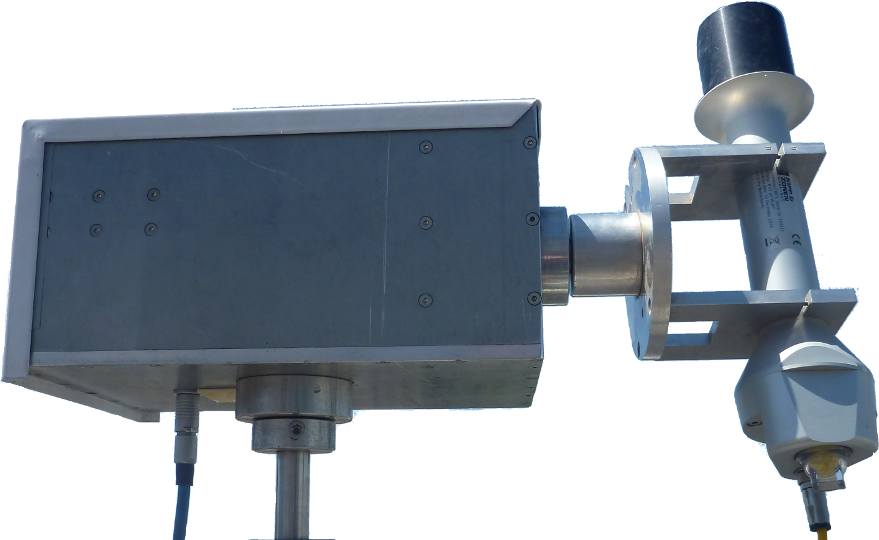
\includegraphics[width=1.0\textwidth]{files/P1110595e2.png}
    \end{figure}
    
\end{topcolumns}%{}

\end{frame}



\begin{frame}%%%%%%%%%%%%%%%%%%%%%%%%%%%%%%%%%%%%%%%%%%%%%%%%%%%%%%%%%%%%%%%%%%%
\frametitle{Ολική Ηλιακή Ακτινοβολίας ευρέους φάσματος}

\begin{topcolumns}%{}

\column{5.5cm}

\begin{figure}
    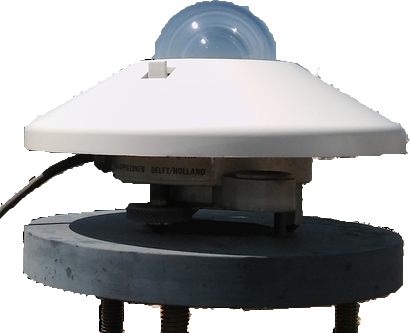
\includegraphics[width=1.0\textwidth]{files/cm21}
\end{figure}

\column{5.5cm}
\begin{block}{Ολική (Global Iradiance)}
    \begin{description}[leftmargin=0em]
        \item[Πυρανόμετρο:] \textbf{CM-21}
        \item[Φάσμα:]       \textbf{335nm - 2200nm}
        \item[Λειτουργία:]  \textbf{από 1993}
    \end{description}
\end{block}
\end{topcolumns}%{}

\end{frame}


\begin{frame}%%%%%%%%%%%%%%%%%%%%%%%%%%%%%%%%%%%%%%%%%%%%%%%%%%%%%%%%%%%%%%%%%%%
\begin{center}
    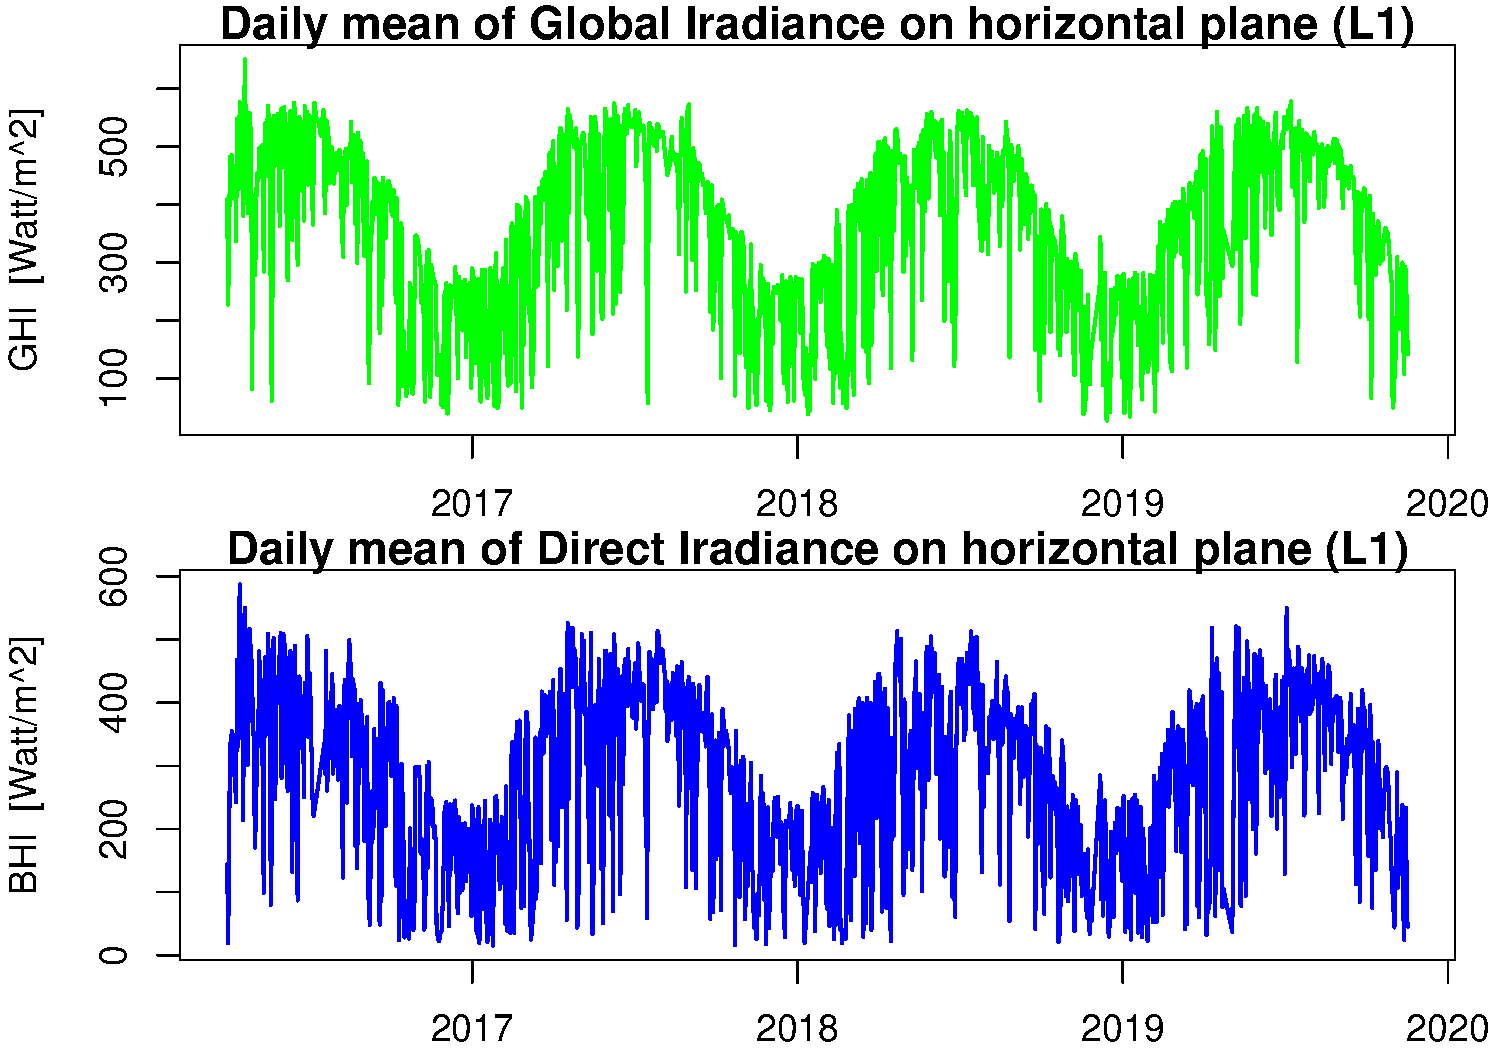
\includegraphics[width=1\textwidth]{files/timeser.pdf}
\end{center}
\end{frame}





\begin{frame}%%%%%%%%%%%%%%%%%%%%%%%%%%%%%%%%%%%%%%%%%%%%%%%%%%%%%%%%%%%%%%%%%%%
\frametitle{Διαχείριση και προετοιμασία δεδομένων}
\framesubtitle{Θέματα που αντιμετωπίσαμε \ldots}

    \begin{itemize}
        \item <1->Έλεγχος και προγραμματισμός λειτουργίας \textbf{ηλιοστάτη}
        \item <2->\textbf{Καθαρισμός} εσφαλμένων καταγραφών
        \item <3->Επιθεώρηση δεδομένων (\textbf{data screening})
        \item <4->Παραγωγή μετρούμενων φυσικών μεγεθών (\textbf{DHI, GNI})
        \begin{itemize}
            \item Σήμα σκότους
            \item Συντελεστής βαθμονόμησης
        \end{itemize}
        \item <5->Αλγόριθμος \textbf{Ποιοτικού Ελέγχου} δεδομένων ακτινοβολίας ``QCRad''
        \item <6->Εντοπισμός/Καθορισμός συνθηκών ``\textbf{καθαρού ουρανού}''
        \item <7->Εύρεση \textbf{δεδομένων} μετεωρολογικών συνθηκών
    \end{itemize}

\end{frame}



\begin{frame}%%%%%%%%%%%%%%%%%%%%%%%%%%%%%%%%%%%%%%%%%%%%%%%%%%%%%%%%%%%%%%%%%%%
\frametitle{Παράδειγμα εντοπισμού "καθαρού ουρανού"}
\framesubtitle{still not perfect \ldots}
\begin{center}
    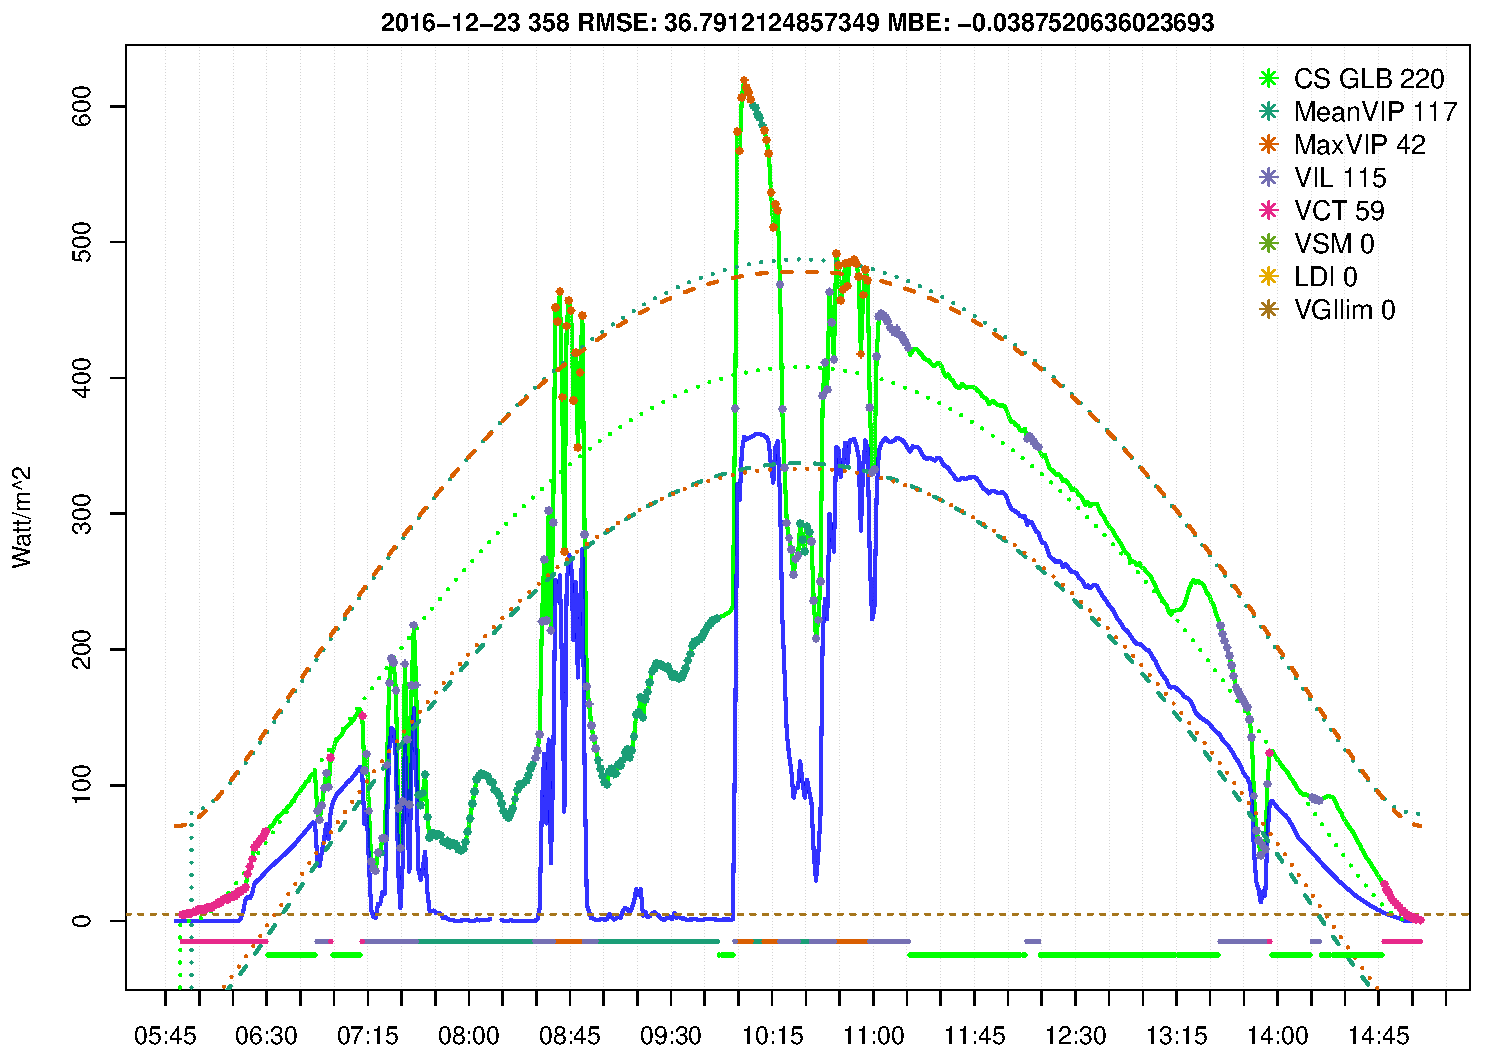
\includegraphics[width=.92\textwidth]{files/CS_827.pdf}
\end{center}
\end{frame}






\begin{frame}%%%%%%%%%%%%%%%%%%%%%%%%%%%%%%%%%%%%%%%%%%%%%%%%%
\frametitle{Προϊόντα και περαιτέρω μελέτη I}
\framesubtitle{or work in progress...}

    \begin{itemize}
         \item <1->\textbf{Άμεση, Ολική} και \textbf{Διάχυτη} Ηλιακή ακτινοβολία ευρέος φάσματος
         \begin{itemize}
             \item Μελέτη τάσεων
             \item Μελέτη εποχικότητας
         \end{itemize}
         \item <2->Παράμετρος \textbf{Linke} για Θεσσαλονίκη
         \item <3->\textbf{Μοντέλο διάχυτης / ολικής} ακτινοβολίας
            \begin{itemize}
                \item Ενεργειακός χαρακτηρισμός
                \item Πρόβλεψη ηλιακού δυναμικού
            \end{itemize}
            \end{itemize}
\end{frame}


\begin{frame}%%%%%%%%%%%%%%%%%%%%%%%%%%%%%%%%%%%%%%%%%%%%%%%%%
\frametitle{Προϊόντα και περαιτέρω μελέτη II}
\framesubtitle{or work in progress...}
    \begin{itemize}

         \item <1->\textbf{Προσομοίωση} μετρήσεων με RTM (libRadTran)
            \begin{itemize}
                \item Επίδραση άλλων παραγόντων / παραμέτρων 
            \end{itemize}
         \item <2->\textbf{Σύγκριση} ``ολοφασματικού'' \textbf{ΑΟD} με φασματικό AOD
         \item <3->Βαθμονόμηση με \textbf{Langley}
            \begin{itemize}
                \item Σύγκριση με Extraterrestrial Solar Constant
            \end{itemize}
         \item <4->Περιγραφή του ρόλου των \textbf{νεφών}
         \begin{itemize}
            \item Συσχέτιση με \textbf{IR} ακτινοβολία
            \item Αναγνώριση από \textbf{Sky Camera}
         \end{itemize}
    \end{itemize}

\end{frame}


\begin{frame}%%%%%%%%%%%%%%%%%%%%%%%%%%%%%%%%%%%%%%%%%%%%%%%%%%%%%%%%%%%%%%%%%%%
\frametitle{Περίληψη}


\begin{itemize}
    \item <1->Περιγραφή της σχέση άμεσης/διάχυτης ακτινοβολίας και των παραγόντων που την καθορίζουν.
    \item <2->Ανάπτυξη μεθόδων και τεχνικών κατάλληλες για τις συνθήκες της Θεσσαλονίκης.
    \item <3->Μελέτη του φυσικού μηχανισμού επίδραση νεφών, aerosol \ldots
\end{itemize}


\end{frame}


\begin{frame}%%%%%%%%%%%%%%%%%%%%%%%%%%%%%%%%%%%%%%%%%%%%%%%%%%%%%%%%%%%%%%%%%%%

\begin{center}
    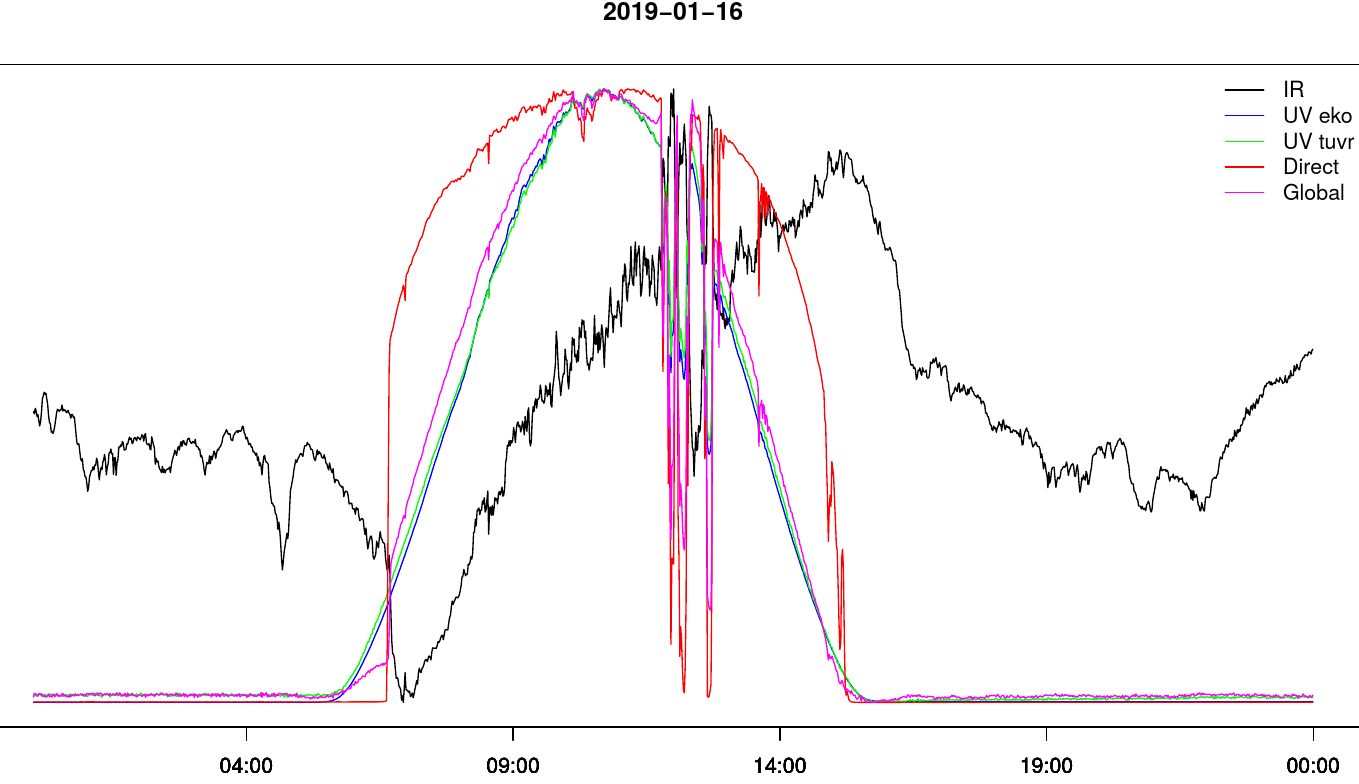
\includegraphics[width=.99\textwidth]{files/multiplot.png}
    \vfill
    {\color{blue} {\Large \textbf{Ευχαριστώ για την προσοχή σας!}}}
\end{center}


\end{frame}








\end{document}
